\documentclass[10pt]{article}
\usepackage[T1]{fontenc}
\usepackage{lmodern,amsmath,amssymb,graphicx,hyperref}
\usepackage[margin=.74in]{geometry}
\setlength{\parindent}{0pt}\setlength{\parskip}{7pt}
\begin{document}
\begin{center}{\Large Uniform odd content and integral factor rescaling}\\[4pt]
Local continuation --- 15 November 2026\end{center}
\textbf{Result.} For the actual single-anchor multiplicity profile
$m_j=\mathbf1_{j=i}$, node $t=-2^i$ and $i<u\le a$, every admissible
odd right factor has coefficientwise two-adic content at least two:
\[
 \operatorname{Content}_2 R_{(r,2b+1),y}(Z)
 \quad\text{for all }r\in\operatorname{Fin}(2^u),\ y\in\operatorname{Fin}(2^a),\quad 2b+1<k.
\]
This is the full polynomial and every column, with the noncrossing zero
branch explicit. No favorable valuation witness is supplied [pcc:unverified].

\textbf{Actual derivation.} Replace the moment variable $H$ by $H/2$.
The actual denominator is quadratic in $H$. Its even coefficients are
integral, while its odd coefficient has content two. The half-slopes
$f=2^{u-1}/(-2^i-\delta)$ and $g=2^{u-1}/(2^i-\delta)$ satisfy
$v_2(f+g)\ge2$ under the actual retained-bit guard. The actual chart slope
has valuation at least two. The diagonal case, unequal-port denominator
valuations and nonzero conditions are derived separately [pcc:unverified].

Coefficientwise parity content is closed under addition, multiplication,
powers and finite sums. Apply it to the actual finite geometric inverse
and the actual integral numerator. Polynomial composition gives the
normalization factor $2^{-b}$ in coefficient $H^b$, yielding the full
odd-factor statement. Standard polynomial and valuation algebra is reused;
no arithmetic novelty is claimed [pcc:unverified].

\textbf{Constructed rescaling.} For odd labels define
\[
 \widetilde L_{x,(r,b)}=4L_{x,(r,b)},\qquad
 \widetilde R_{(r,b),y}=\tfrac14R_{(r,b),y};
\]
keep even labels unchanged. The right factors remain integral. The actual
weighted left content changes from $w+b$ to $w+b+2$ on odd labels.
The selected-node weight $w=a+1-i+G_i(m)$ is nonnegative for this profile,
so the left factors are integral too [pcc:unverified].

The source proves the exact identities and unchanged residual
\[
 \widetilde L\widetilde R=LR,\qquad
 \operatorname{Content}_{w+k}\bigl(W_{\rm crossing}-\widetilde L\widetilde R\bigr).
\]
Scaling occurs in rational polynomials before finite-ring reduction; it
uses no inverse of four in a ring of characteristic $2^p$. Every
$2^u k$ label is retained. These are the same auxiliary crossing matrix
and residual, not a replacement elliptic relation map [pcc:unverified].
\newpage
\begin{center}{\Large Admission, evidence and continuation}\end{center}
\textbf{Global schedule test.} The original schedule is
\[
 G_j(m)=m_j-\sum_{s<u}(s-j)_+m_s.
\]
For the actual single-anchor profile, the separate admission run derives
\[
 G_j(\mathbf1_i)=\mathbf1_{j=i}-(i-j)_+\quad(i<u).
\]
Thus $G_j=-(i-j)<0$ whenever $j<i$. For $i>0$ this profile fails the
all-node nonnegativity premise of the existing schedule interface.
At $i=0$, all retained schedules are nonnegative. This checks that one
premise only; child interfaces and a common global construction still
require separate work [pcc:unverified].

\begin{center}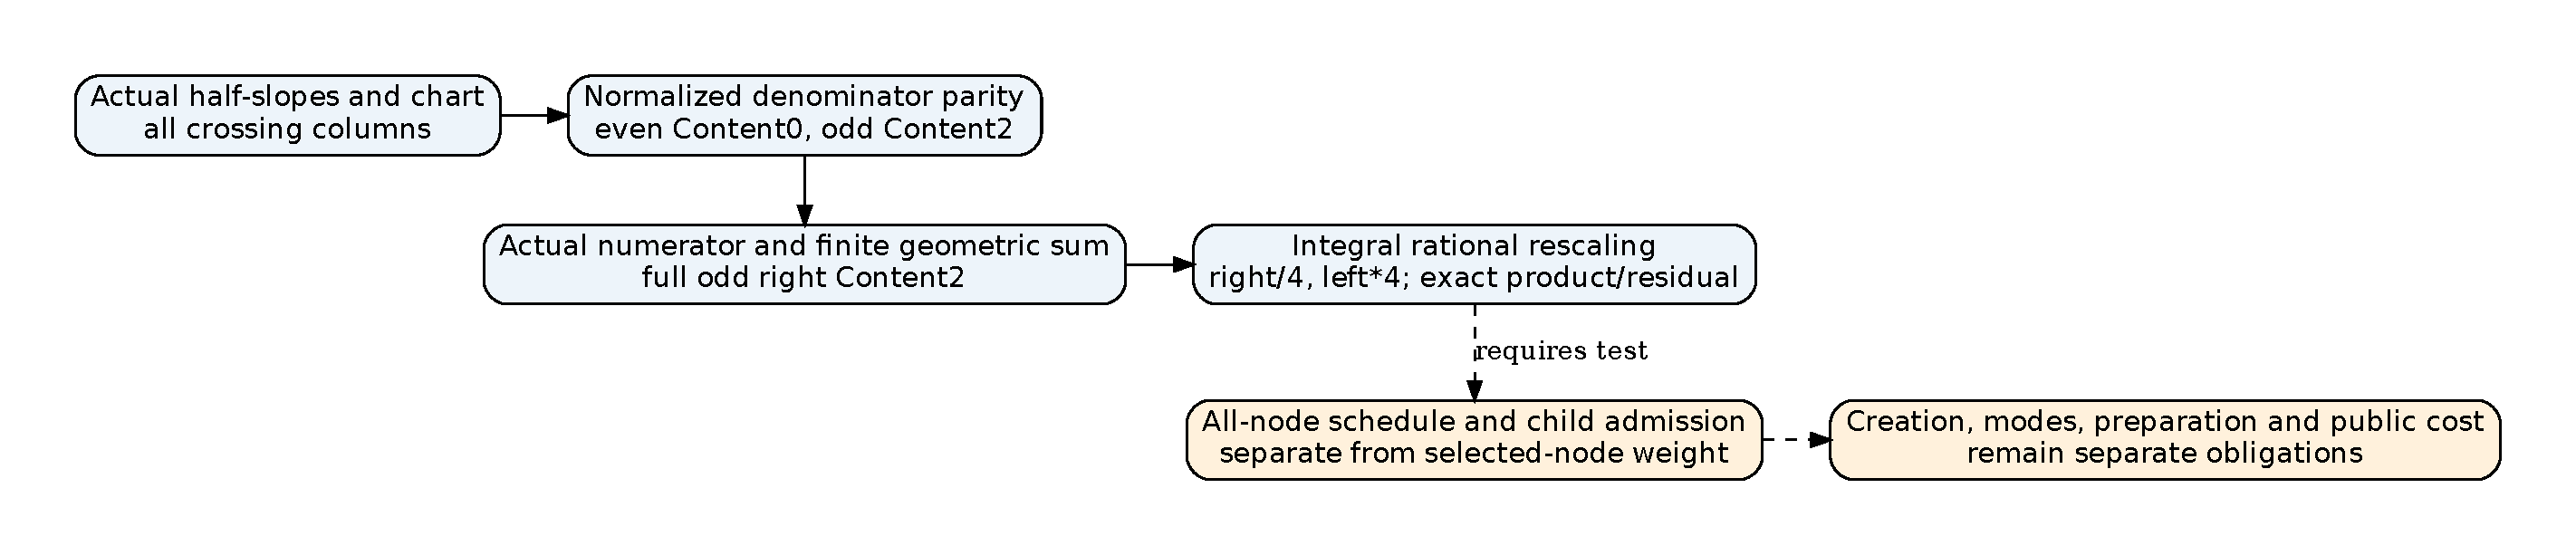
\includegraphics[width=\linewidth,height=2.65in,keepaspectratio]{uniform-rescaling-dependencies-001.pdf}\end{center}
\textbf{Evidence.} Accepted088 has411 local theorem statements including
parent397;090 has418;093 has428. All three exit zero without warnings or
sorryAx. Receipts044--046 bind the exact source, raw compiler output and
exit files. Printed central dependencies are standard. Failed087,089,091
and092 are retained. Admission094 had lexical errors;095 attempted an absent source after an administrative path failure;096 passed with a deprecated lemma warning. Accepted097 replaces that lemma and has432 statements including428, exit zero without warnings;receipt047 pins it. These raw failures are retained. This evidence is outside shared Transport53/57/fresh;
all new claims are unsigned and defaultnot\_covered [pcc:unverified].

\textbf{Sources and interpretation.} Exact primary sources are
\texttt{OrientationAnchor.schedule},
the actual schedule feasibility theorem in \texttt{OrientationBudget}, the earlier
jet-completion proposal, its rank-directed backlog and pole-correction
report. The KB was unavailable; committed source hashes are recorded in the accompanying source-review JSON. The prior bounded search remains
unlaunched. A finite weight shift alone does not establish a new asymptotic
exponent. No timing or CPU-isolation inference is made from exact algebra.

\textbf{Next technical step.} Test a common multiplicity profile that admits
all retained nodes while retaining the derived odd-content bound. Charge
its actual degree and all child interfaces. Original creation precision,
mode inventory, coefficient preparation and complete public bit costs
remain separate obligations. No native, timing, scaling, paid/cloud or
attack campaign was run. Existing checkpoint artifacts remain unchanged.
\end{document}
